\section{Anhang}

\subsection{Projektmanagement}

\bild{1}{timeline}{Meilenstein Planung}

\begin{longtable}{l l l}
	\hline
	\textbf{MS} & \textbf{Datum} & \textbf{Inhalt} \\
	\hline

	1	& 27. Februar 	& 
	\begin{tabular}[t]{@{} l @{}}
		\tabitem Kick-Off Meeting \\
		\tabitem Besprechung von Aufgabenstellung \\
		\tabitem Projektvorgehen und Meetings besprechen \\
	\end{tabular} \\
	\hline

	2	& 13. März 		& 
	\begin{tabular}[t]{@{} l @{}}
		\tabitem Projekt- und Risikomanagement \\
		\tabitem Grobplanung Projektablauf (Meilensteine) \\
		\tabitem Grobkonzept (grobe Erfassung Fragestellungen, Scope, Anforderungen) \\
		\tabitem Grundaufbau Dokumentation \\
	\end{tabular} \\
	\hline

	3	& 8.  Mai 		& 
	\begin{tabular}[t]{@{} l @{}}
		\tabitem Besprechung Ideenfindung \\
		\tabitem Recherche von Swift und den relevanten Frameworks \\
		\tabitem Technische Grenzen definiert \\
		\tabitem Mehrere Problemlösungszyklen durchlaufen \\
		\tabitem Prototypen zu den Problemlösungszyklen \\
		\tabitem (funktionale) Anforderungen festgelegt \\
		\tabitem Planung der Umsetzung, Arbeitspakete \\
	\end{tabular} \\
	\hline

	4	& 22. Mai 		& 
	\begin{tabular}[t]{@{} l @{}}
		\tabitem Testatsitzung \\
		\tabitem Besprechung erreichter Ziele \\
		\tabitem funktionierende App, die min. alle Muss-Anforderungen erfüllt \\
		\tabitem Entwurf der abzugebenden Dokumentation \\
	\end{tabular} \\
	\hline

	5	& 8.  Juni 		& 
	\begin{tabular}[t]{@{} l @{}}
		\tabitem Abgabe Projekt \\
		\tabitem fertige Dokumentation \\
		\tabitem fertige App \\
		\tabitem Entwurf Schlusspräsentation \\
	\end{tabular} \\

	\hline
	\caption{Auflistung der Meilensteine}
	\label{tab:meilensteine}
\end{longtable}


\subsection{Problemlösungszyklus}
Die definierten Problemstellungen und Ideen von der Ideenfindungsphase werden mit dem explorativem Verfahren in der Ideenauswahlphase mittels dem Problemlösungszyklus evaluiert. Der Zyklus setzt sich aus den Phasen Problemdefinitionen, Needs, Ideen, Prototypen \& Storytelling und Testen zusammen.

\bild{1}{problemloesungszyklus}{Problemlösungszyklus}



\subsection{Aufgabenstellung}
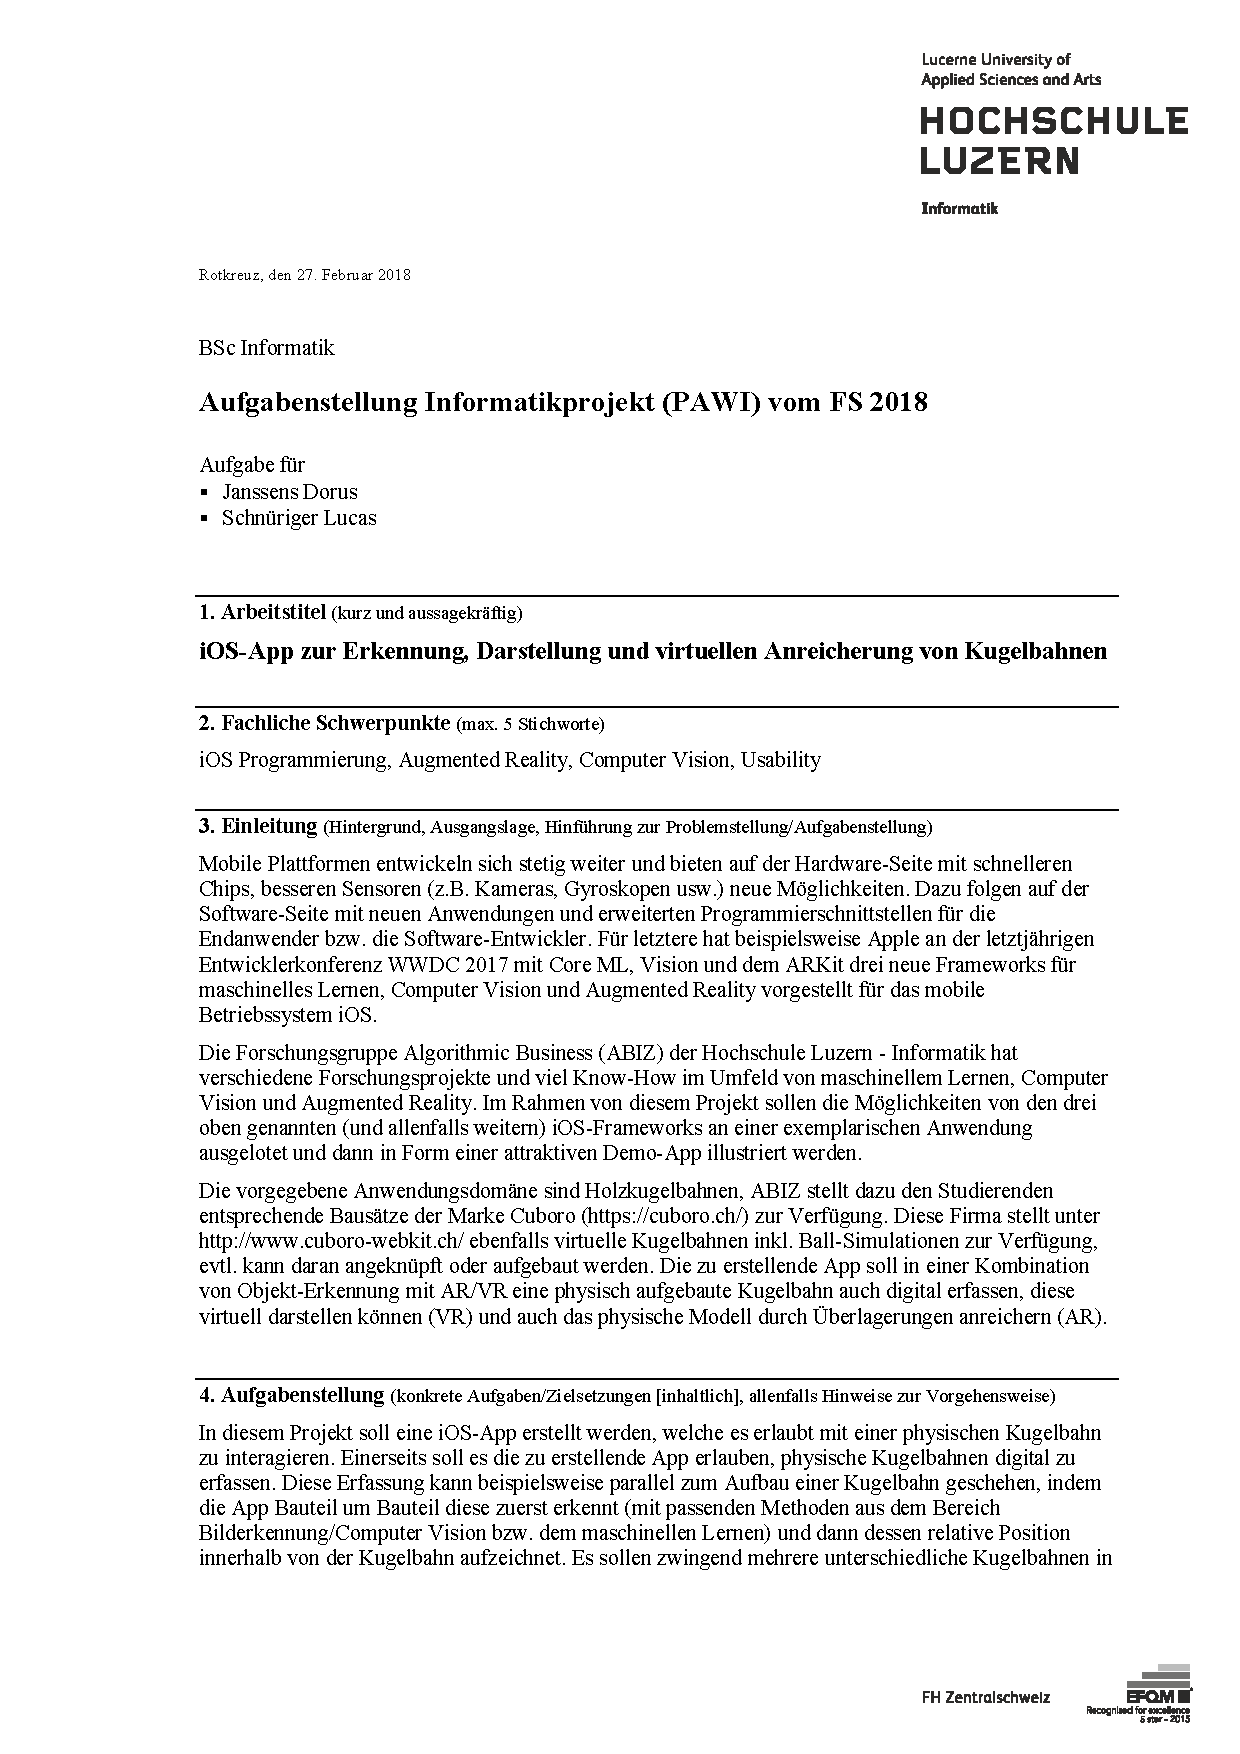
\includepdf[pages=-]{appendix/Aufgabenstellung_PAWI_FS_2018_Janssens_Schnueriger.pdf}

\IfFileExists{99-Protokolle}{
	\newpage
	\subsection{Protokolle}

\setlist[itemize]{noitemsep}

\subsubsection*{22.05.2018 - Sitzung}

Anwesend: Ruedi Arnold, Lucas Schnüriger, Dorus Janssens

\textbf{Fragen}
\begin{itemize}
	\item Demo-App: Rotation um nur eine Achse auch akzeptabel?
	\begin{itemize}
		\item Noch einmal eine Stunde investieren, um zu sehen, ob die Rotation um alle drei Achsen nicht doch geht, bspw. mit einer Transformationsmatrix
	\end{itemize}
	\item Dokumentation:
	\begin{itemize}
		\item Wie sollen die (funktionalen) Anforderungen festgehalten werden: Teil des Hauptteil (Problemstellung) oder in Anhang (Architekturdokumentation)?
		\item Anforderungen können im Anhang gehandhabt werden. Sie sollen aber nicht doppelt aufgeführt werden.
	\end{itemize}
	\item Prototypen: die Fragestellungen und Resultate in einer Übersicht sammeln oder Teil der Prototypen Beschreibung oder gar an beiden Stellen?
	\begin{itemize}
		\item Kurze Liste mit Beschreib der Unterfangen, allenfalls Erfüllungsgrad visualisieren (bspw. mit Ampelsystem)
		\item Der bisherige Aufbau zur Beschreibung der Prototypen sonst ist ok
	\end{itemize}
	\item Umfang des Testing: Testplan und Testprotokoll oder einfach Anforderungen validieren? Wie dokumentieren: in Hauptteil/Anhang?
	\begin{itemize}
		\item Anforderungen validieren anhand der Akzeptanzkriterien, Erfüllungsgrad prüfen und Unvollständigkeiten begründen
		\item Festhalten im Hauptteil unter "Validierung" passt
		\item Unit Tests nicht notwendig
	\end{itemize}
\end{itemize}

\textbf{Weitere Arbeitsschritte / zu bearbeitende Fragestellungen}
\begin{itemize}
	\item Demo-App fertigstellen:
	\begin{itemize}
		\item Rotation nochmals überarbeiten und allenfalls darlegen warum es nicht funktioniert
		\item Löschalgorithmus fertig implementieren, sodass keine "Inseln" gebildet werden können
		\item Einen "About"-Bereich ergänzen (mit Name, Version)
		\item Das Schachbrettmuster der Flächenerkennung nach Start Editor/Guide nicht mehr anzeigen, oder transparenter
		\item Methoden der Klasse zur Persistierung statisch machen, nicht als Objekt benötigt
	\end{itemize}
	\item Dokumentation fertigstellen:
	\begin{itemize}
		\item Wichtig: Dokumentation muss eine objektive Bewertung und ein persönliches Fazit (pro Student) enthalten
		\item Die Projektplanung (Grobplan/Meilensteine) kann direkt in den Hauptteil der Dokumentation unter "Problemstellung"
		\item Protokolle, Arbeitsjournale, Risikomanagement im Anhang der Dokumentation mit abgeben aber nicht ausdrucken
		\item Aufgabestellung in den Anhang, Einleitung/Ausgangslage mit eigener Formulierung
		\item Source Dateien im Anhang (nicht nur von Prototypen/App, sondern auch von Bildern, Grafiken und Diagrammen)
		\item Den Backlog wenn möglich anhängen (vom GitHub Project nach Möglichkeit exportieren)
	\end{itemize}
	\item Demo Video erstellen
\end{itemize}

\textbf{Varia}
\begin{itemize}
	\item Zum letzten Statusprotokoll: der 1. und 3. Arbeitsschritt aus "Stand der Arbeit" würde in "Ausgeführte Arbeiten" kommen, "Stand der Arbeit" sollte SOLL-IST vergleichen
	\item Demo-App wurde vorgeführt, die App wurde zudem auf Herr Arnolds Gerät installiert
	\item Abgabe nicht auf CD notwendig, kann bspw. auch als Dropbox Link sein
	\item Arnold ist bis nächste Woche noch per Mail erreichbar, in Kalenderwoche 23 (4.-8. Juni) abwesend
	\item erhalten, Termin für Präsentation haben wir anschliessend an die Sitzung erhalten: 25. Juni, 14.00 Uhr)
\end{itemize}


\subsubsection*{08.05.2018 - Sitzung}

Anwesend: Ruedi Arnold, Lucas Schnüriger, Dorus Janssens

\textbf{Weitere Arbeitsschritte / zu bearbeitende Fragestellungen}
\begin{itemize}
	\item Demo App umsetzen
	\begin{itemize}
		\item englische Benutzeroberfläche, Mehrsprachigkeit nicht notwendig
		\item Architektur auf Basis VIPER ist ok, einfach nicht zuviel "Overhead" erzeugen, ein bottom-up Ansatz wäre auch ausreichend -> am Schluss ist die Funktionalität wichtig
	\end{itemize}
	\item Anforderungen in Dokumentation fertigstellen / Korrekturen anbringen:
	\begin{itemize}
		\item User Stories fortlaufend, bzw. eindeutig nummerieren
		\item bei Bauanleitung von "Schritten" nicht "Elementen" reden
		\item Anzahl integrierte Elemente: "mindestens" 4 schreiben
		\item Erstellen neuer Kugelbahn: ergänzen, dass man die Kugelbahn benennen kann, unter einem Namen speichert
		\item Platzieren neuer Element im Editor: präzisieren, wo das Platzieren möglich ist (nur valide Positionen)
		\item zusätzliche Soll oder Kann Anforderung zur Umbenennung von gespeicherten Kugelbahnen
		\item Ändern der Ausrichtung eines Element im Editor: spezifizieren, dass nur um 90° entlang der drei Achsen gedreht wird
		\item allg. Formulierungen kontrollieren und präzisieren wo nötig, darauf achten, dass sie unmissverständlich sind 
	\end{itemize}
	\item Mockups (UI):
	\begin{itemize}
		\item AR Screen überdenken: bspw. eine Navigationsbar oben inkl. zurück-Button und deutlicher Anzeige welcher Modus aktiv ist, was der nächste Schritt für den User ist (bspw. "Fläche auswählen")
		\item im Build Mode das aktuelle Element anzeigen, damit klar ist, welcher virtueller Würfel als nächstes gesetzt wird
	\end{itemize}
	\item Konzept für Demo Video erstellen
\end{itemize}

\textbf{Varia}
\begin{itemize}
	\item Dokumentation:
	\begin{itemize}
		\item Adäquate Deutsche Begriffe Anglizismen vorziehen (bspw. Speicher statt Memory oder Datei statt File)
		\item Begriffe konsistent/einheitlich verwenden
	\end{itemize}
	\item Die beiden Modi der App passender benennen:
	\begin{itemize}
		\item bisherigen Editier Modus als Build Modus, da in diesem Modus virtuelle Bahnen gebaut werden
		\item bisheriger Build Modus als Guide (oder ähnlich), da dies eine Anleitung ist
	\end{itemize}
	\item Laut Herrn Arnold hatte Herr Koller kürzlich wieder Kontakt mit cuboro. Sollten wir in den nächsten Tagen nichts hören, soll um ein Statusupdate bei Herr Koller nachgefragt werden
\end{itemize}


\subsubsection*{23.04.2018 - Sitzung}

Anwesend: Ruedi Arnold, Lucas Schnüriger, Dorus Janssens

\textbf{Weitere Arbeitsschritte / zu bearbeitende Fragestellungen}
\begin{itemize}
	\item Mockups fertigstellen
	\item PDF von den neuen Mockups Herr Arnold zukommen lassen
	\item Min. 4-5 Würfeltypen in die App integrieren
	\item Fertigstellen Konzept Demo-App
	\item Start Umsetzung Demo-App
\end{itemize}

\textbf{Varia}
\begin{itemize}
	\item Constraint setzen beim Löschen der Würfel im Editiermodus, damit keine Inseln gemacht werden können
	\item Demo an Herr Koller zeigen und Nachfragen ob eine Rückmeldung von cuboro eingetroffen ist
	\item Build- und Editiermodus mit visuellen Elementen für den Benutzer eindeutig identifizierbar machen (z.B Farbe)
	\item Mögliche Anschlusspunkte der Würfel hinterlegen und Anzeigen ob die Elemente zusammenpassen
	\item Für das Demo Video kann die Kugel in X- oder Z-Richtung angeschubst werden
	\item Mocks realistischer darstellen ohne Platzhalter  
	\item Simulation mit virtueller Kugel vorsehen (SceneKit Physikengine)
\end{itemize}

\subsubsection*{10.04.2018 - Sitzung}

Anwesend: Ruedi Arnold, Lucas Schnüriger, Dorus Janssens

\textbf{Weitere Arbeitsschritte / zu bearbeitende Fragestellungen}
\begin{itemize}
	\item AR Bauanleitung einer Kugelbahn Würfel-für-Würfel (Fortsetzung vom Prototyp zur Bauanleitung)
	\item Schrittweiser Aufbau einer augmentierten Bahn durch den Benutzer
	\item Korrektur der Position durch manuelles Verschieben der cuboro Bahn und Würfeln
	\item Konzept der Demo-Applikation erarbeiten
\end{itemize}

\textbf{Varia}
\begin{itemize}
	\item If-Else Konstrukt zum Drehen der Würfel in ein Enum oder einer Klasse verpacken (Strategie Pattern)
	\item Hit-Testing dokumentieren und im Ausblick als ein mögliches weiteres Projekt festhalten 
	\item Herr Koller wird von Dorus Janssens im Modul WebLab eine Demo der aktuellen Prototypen erhalten
	\item Für die Demo soll eine kleine Bahn verwendet werden (ca. 4 x 4 Grundfläche)
	\item in 2 Wochen geplantes Ende der explorativen Phase
	\item Neue Anforderung: Demofilm für die Endabgabe
\end{itemize}


\subsubsection*{27.03.2018 - Sitzung}

Anwesend: Ruedi Arnold, Lucas Schnüriger, Dorus Janssens

\textbf{Weitere Arbeitsschritte / zu bearbeitende Fragestellungen}
\begin{itemize}
	\item Vorschlag: Mehrere cuboro Elemente modellieren und eine einfache Bahn vordefinieren und augmentieren. Zweiter Schritt besteht darin mit der augmentierten Bahn zu interagieren.
	\item zu bearbeitende Themen:
	\begin{itemize}
		\item Würfel/Bahn modellieren: lässt sich cuboro-Webkit Export nutzen? Ansonsten cuboro anfragen (via Herr Koller), oder dann selber Wege zur Modellierung finden.
		\item virtuelles Modell einer Bahn auf einen Tisch projizieren
		\item AR Bauanleitung einer Bahn mit schrittweisem Aufbau
		\item erkennen ob sich innerhalb einer Bounding Box ein physischer Würfel befindet
		\item mittels Touchgesten virtuelle Objekte drehen
	\end{itemize}
\end{itemize}

\textbf{Varia}
\begin{itemize}
	\item Herr Arnold stets in CC nehmen bei Mails
	\item Herr Koller anfragen wegen Kontakt zu cuboro: für 3D Modelle der Würfel
	\item Versuche konkret dokumentieren: detailliert die Erkenntnisse, Versuche und Zwischenschritte festhalten; mit Screenshots, Codeausschnitten, Verweise auf Doku; im Hinterkopf behalten, dass damit jemand daran weiterarbeiten könnte, nachvollziehbar machen wieso welche Schritte genommen wurden; was wäre sonst noch möglich, Ausblick, alternative Möglichkeiten die nicht weiterverfolgt wurden
	\item Der Haupttreiber dieser Arbeit ist technisch, \textit{nicht} Business-Case
	\item Mail an Herr Arnold, wenn im GitHub Projects die Versuche erfasst sind
	\item Verweise auf die Projekte, die als Grundlage dienten, sollen im Repo enthalten sein; an passender Stelle (Readme, direkt im Code) erwähnen
\end{itemize}


\subsubsection*{13.03.2018 - Sitzung}

Anwesend: Ruedi Arnold, Lucas Schnüriger, Dorus Janssens

\textbf{Fragen}
\begin{itemize}
	\item Können wir die Einleitung und Aufgabenstellung in der erhaltenen Form verwenden?
	\begin{itemize}
		\item Die Einleitung und Aufgabenstellung können aktuell so beibehalten werden und gegen Ende des Projekts genauer spezifiziert werden.
	\end{itemize}
	\item Wie werden die funktionalen Anforderungen im explorativen Verfahren gehandhabt?
	\begin{itemize}
		\item Z.B. Overlays als Anforderung definieren und im Verlauf des Problemlösungszyklus einzelne Funktionalitäten näher festlegen.
		\item Somit ergeben sich grobe Anforderungen zu Beginn des Projektes und genauer spezifizierte Anforderungen nach dem Erkenntnisgewinn.
	\end{itemize}
	\item Planung / Vorgehen und Dokumentation bei explorativem Verfahren?
	\begin{itemize}
		\item Die Phasen Ideenfindung und Ideenauswahl zusammenlegen, sie laufen in kleineren Zeitrahmen immer wieder ab.
		\item Problemlösungszyklen einzeln dokumentieren und den Erkenntnisgewinn ausführlich formulieren.
	\end{itemize}
	\item In welcher Phase läuft der Problemlösungszyklus?
	\begin{itemize}
		\item Da die Ideenfindung und Ideenauswahl zusammengelegt wird ist dies ständig der Fall.
	\end{itemize}
\end{itemize}

\textbf{Weitere Arbeitsschritte / zu bearbeitende Fragestellungen}
\begin{itemize}
	\item Wie kann ein Overlay auf einem physischen Würfel erzeugt werden?
	\begin{itemize}
		\item Das SceneKit eignet sich für 3D Objekte und das SpriteKit für 2D Flächen. Welches ist passender?
	\end{itemize}
	\item Wie können physische Körper als virtuelle Objekte modeliert werden?
\end{itemize}

\textbf{Varia}
\begin{itemize}
	\item Öfters Prototypen oder ähnliches kommunizieren
	\item Ein Overlay auf einem Würfel erzeugen ist aktuell priorisiert
	\item Die Technischenaskpekte und Umsetzung stehen im Vordergrund
	\item Die Dokumentation soll vor allem die technische Funktionsweise (relevanter, wesentlicher Code) und neue Erkenntnisse aufzeigen
\end{itemize}

\subsubsection*{27.02.2018 - Kick-Off Meeting}

Anwesend: Ruedi Arnold, Lucas Schnüriger, Dorus Janssens

\begin{itemize}
	\item Herr Arnold hat uns den Sachverhalt des Projekts erklärt.
	\item Die Aufgabenstellung ist bewusst offen, es sollen die Möglichkeiten der AR Technologie mit Apples ARKit ausgelotet werden.
	\item Alle zwei Wochen wird ein Meeting abgehalten. Das Meeting findet jeweils 10:00 bis 11:00 statt.
	\item Falls benötigt kann ein iOS Gerät zur Verfügung gestellt werden.
	\item Das Projekt wird im explorativem Verfahren gehandhabt.
	\item Ein Set einer Cuboro Kugelbahn steht bei Herrn Thomas Koller zur Verfügung.
\end{itemize}


}

\IfFileExists{99-Risikomanagement}{
	\newpage
	\subsection{Risikomanagement}

\begin{longtable}{lp{3.5cm}lllp{3.5cm}p{3.5cm}}
	\hline
	\textbf{Nr.} & \textbf{Beschreibung} & \textbf{W} & \textbf{A} & \textbf{W*A} & \textbf{Prävention} & \textbf{Reaktion} \\ 
	\hline
	01  & Ausfall eines Projektmitarbeiters & 1 & 2 & 2 & Regelmässiger Wissensaustausch und Projektmeetings, zentrale Dokumentation aller Vorgänge (GitHub) & Betreuenden Dozenten informieren und Anforderungen einschränken \\
	\hline
	02  & Projektdaten gehen verloren & 0 & 3 & 0 & Daten regelmässig sichern, Daten versionisiert auf GitHub & Daten wiederherstellen \\
	\hline
	03  & GitHub fällt aus & 1 & 1 & 1 & lokale Kopien aller Daten & auf lokalen Kopien arbeiten und auf HSLU GitLab migrieren \\
	\hline
	04  & Anforderungen werden nicht erfüllt & 1 & 2 & 2 & regelmässiges Überprüfen / Meetings mit betreuendem Dozenten, realistische Ziele setzen & Rechtzeitige Information an Projektbeteiligte und Anpassung des Projektplans \\
	\hline
	05  & Zeitaufwand und Komplexität für Entwicklung zu hoch & 1 & 3 & 3 & eingehende Technologierecherche und Versuche & Betreuenden Dozenten informieren, um Hilfe bei Dozenten suchen, Anforderungen einschränken \\
	\hline
	06  & Frameworks weisen nicht die funktionalen Anforderungen auf die im Marketing versprochen werden. & 1 & 3 & 3 & Mittels Problemlösungszyklen die Funktionalität überprüfen und verifizieren & Rücksprache mit dem Auftraggeber und dem Betreuer \\
	\hline
	07  & Beschränkte Erfahrung mit iOS und Swift erhöht die Zeit der Evaluation und gefärdet somit den tiefe Grad der Problemlösungszyklen. & 1 & 3 & 3 & Genügend Zeit bei den ersten Problemlösungszyklen definieren & Anpassung der Anforderungen und Rücksprache mit dem Auftraggeber und dem Betreuer \\
	\hline
	08  & Betas von ARKit 1.5 oder iOS 11.3 sind instabil oder ändern genutzte Funktionen & 0 & 2 & 0 & Known Issues recherchieren, Verwendung von neuen Funktionen bewusst wählen und Alternativen berücksichtigen & Issue an Apple reporten, an anderen (gleich wichtigen) Aufgaben arbeiten, alternative Methoden suchen, auf stabile Funktionen zurückgreifen \\
	\hline
	09  & Leistung der (Test)Geräte nicht ausreichend & 1 & 2 & 2 & Technologische Anforderungen (welche Generation von iPhones/iPads) in der Recherche berücksichtigen, beim Bau von Prototypen Zeit einplanen zu Performance Tests & Code/Methoden optimieren, alternative Lösungen weiterverfolgen \\
	\hline
	10  & Präzision des Tracking zu niedrig um das Cuboro Element sicher zu Tracken & 2 & 2 & 4 & Anforderungen mit einem Tolleranzbereich definieren. & Marker anbringen um die präzision des Trackings zu erhöhen. Third party Software zur erkennung des Würfels verwenden. \\
	\hline
	11  & Präzision der Hit-Tests zu niedrig um zu ermitteln ob sich ein physisches Objekt in einer augmentierten Bounding Box befindet & 2 & 2 & 4 & Bestätigen mittels einer Tapgeste oder einem Button klick. & Verschiedene Versuche durchführen um die Genauigkeit zu ermitteln. \\
	\hline
	12  & Erhalten keine oder nicht verwendbar 3D Daten von cuboro Elemente & 1 & 2 & 2 & Kontakt mit cuboro herstellen & Einfache Würfel als Platzhalter, eigene einfache Elemente mit SceneKit oder Drittanbieter Software (bspw. Blender) erstellen \\
	\hline
	13  & Präzision des Worldtrackings ist zu instabil um die Bahn auf der ausgewählten Fläche zu halten & 2 & 2 & 4 & ARKit 1.5 nutzen & Funktion um die Bahm manuell zu korrigieren \\
	\hline
	14  & Korrekte Rotation der Elemente zu komplex & 2 & 2 & 4 & - & Anzahl Rotationsachsen verringern \\
	\hline
	15  & Worldtracking bei Unterbrüchen zu instabil & 2 & 2 & 4 & Unterbrüche der Szene vermeiden & Popup statt Modal verwenden um keinen Unterbruch zu erzeugen, Benutzer über Relokalisierung informieren \\
	\hline
\end{longtable}

\textbf{Legende}
\begin{itemize}
	\item \textbf{W:} Wahrscheinlichkeit
	\item \textbf{A:} Auswirkungen
\end{itemize}

\subsubsection*{Änderungsprotokoll}

\begin{table}
	\begin{tabular}{llp{10cm}}
		\hline
		\textbf{Datum} & \textbf{Autor} & \textbf{Bemerkungen} \\
		\hline
		06.03.2018 & Lucas & Erstellung der Tabelle mit Risiken 01-05 \\
		10.03.2018 & Dorus & Erweiterung um Risiken 06-07 \\
		12.03.2018 & Lucas & Erweiterung um Risiken 08-09 \\
		26.03.2018 & Lucas \& Dorus & Erweiterung um Risiko 10 \\
		26.03.2018 & Dorus & Risiko 07 W heruntergestuft von 2 auf 1 \\
		09.04.2018 & Dorus & Erweiterung um Risiko 11 \\
		09.04.2018 & Lucas & Risiko 08 W heruntergestuft von 1 auf 0, iOS 11.3 / ARKit 1.5 sind veröffentlicht \\
		22.04.2018 & Lucas & Erweiterung um Risiko 12 \\
		22.04.2018 & Lucas \& Dorus & Erweiterung um Risiko 13 \\
		07.05.2018 & Lucas & Risiko 10 heruntergestuft von 3 auf 2 \\
		07.05.2018 & Lucas & Risiko 12 heruntergestuft von 2 auf 1 \\
		21.05.2018 & Lucas \& Dorus & Erweiterung um Risiken 14-15 \\
		\hline
	\end{tabular}
\end{table}


}

\IfFileExists{99-Arbeitsjournale}{
	\newpage
	\subsection{Arbeitsjournale}

\subsubsection{Arbeitsjournal von Dorus Janssens}

% TODO:

\subsubsection{Arbeitsjournal von Lucas Schnüriger}

% TODO:

}

\IfFileExists{99-Architektur}{
	\newpage
	\section{Architekturdokumentation}\label{appendix:architekturdokumentation}

Die folgende Architekturdokumentation wurde parallel zum Projekt im Rahmen des Moduls Softwarearchitektur, -qualität und Testing (SAQT) an der Hochschule Luzern erarbeitet.

\subsection{Funktionale Anforderungen}\label{appendix:funktionale-anforderungen}
\subsubsection{Epics}
Die App soll folgende \textbf{Epics} erfüllen:
\begin{enumerate}
	\item \textbf{Bauanleitung (Guide):} Der Benutzer kann von einer gewählten Kugelbahn eine Augmented Reality Bauanleitung erhalten, um die Bahn physisch nachbauen/aufbauen zu können.
	\item \textbf{Baumodus (Builder):} Der Benutzer kann in Augmented Reality eine virtuelle Kugelbahn neu erstellen oder eine bestehende verändern, damit diese als Bauanleitung zur Verfügung stehen.
\end{enumerate}

\subsubsection{User Stories}\label{appendix:user-stories}

\begin{longtable}{l l p{13cm}}
	\hline
	\textbf{Nr.} & \textbf{Prio.} & \textbf{Beschreibung} \\
	\hline
	\textbf{1} & & \textbf{Allgemein} \\
	\hline
	1.1 & M &
		\begin{tabular}[t]{@{}p{13cm}@{}}
			Als Benutzer kann ich eine Fläche der realen Welt als Ebene für Augmented Reality auswählen, damit diese als Basis für die Anwendung verwendet wird. \\
			Akzeptanzkriterien:
			\begin{itemize}
				\item Von ARKit erkannte Flächen werden als rechteckige Flächen dargestellt.
				\item Durch antippen einer Fläche wird diese ausgewählt und alle anderen Flächen ausgeblendet und gelöscht.
				\item Die vertikale Position einer neu zu setzenden Kugelbahn orientiert sich an der ausgewählten Fläche, bzw. kommt darauf zu stehen.
			\end{itemize} \vspace*{-\baselineskip}
		\end{tabular} \\
	\hline
	1.2 & M &
		\begin{tabular}[t]{@{}p{13cm}@{}}
			Als Benutzer kann ich eine Kugelbahn auf der ausgewählten Ebene platzieren. \\
			Akzeptanzkriterien:
			\begin{itemize}
				\item Wenn eine Fläche ausgewählt ist, wird darauf eine Kugelbahn angezeigt.
				\item Die Kugelbahn befindet sich stets zentral im Kamerabild auf der Fläche.
				\item Durch Benutzereingabe, kann die Bahn an der aktuellen platziert werden.
			\end{itemize} \vspace*{-\baselineskip}
		\end{tabular} \\
	\hline
	1.3 & M & 
		\begin{tabular}[t]{@{}p{13cm}@{}}
			Als Benutzer kann ich die Kugelbahn auf einer Fläche ausrichten, damit sie wie gewünscht positioniert ist. \\
			Akzeptanzkriterien:
			\begin{itemize}
				\item Die Kugelbahn ist während des Platzierens stets zur Kamera ausgerichtet, sodass eine Drehung des Geräts auch die Rotation der Kugelbahn gegenüber der realen Welt verändert.
			\end{itemize} \vspace*{-\baselineskip}
		\end{tabular} \\
	\hline
	1.4 & M & 
		\begin{tabular}[t]{@{}p{13cm}@{}}
			Als Benutzer will ich erkennen in welchem Modus (Bauanleitung, Editor) ich mich befinde. \\
			Akzeptanzkriterien:
			\begin{itemize}
				\item Auf dem AR Bildschirm wird unmissverständlich angezeigt, welcher Modus aktiv ist.
			\end{itemize} \vspace*{-\baselineskip}
		\end{tabular} \\
	\hline
	1.5 & S & 
		\begin{tabular}[t]{@{}p{13cm}@{}}
			Als Benutzer kann ich die Position und Ausrichtung einer Kugelbahn korrigieren, damit sie mit der physischen Kugelbahn übereinstimmt. \\
			Akzeptanzkriterien:
			\begin{itemize}
				\item Die Position der Kugelbahn lässt sich über Bedienelemente in Richtung aller drei Achsen verschieben.
			\end{itemize} \vspace*{-\baselineskip}
		\end{tabular} \\
	\hline
	1.6 & K & 
		\begin{tabular}[t]{@{}p{13cm}@{}}
			Als Benutzer kann ich zwischen den Modi wechseln, damit ich die aktuelle Bahn im anderen Modus direkt weiterverwenden kann. \\
			Akzeptanzkriterien:
			\begin{itemize}
				\item Es besteht die Möglichkeit den aktiven Modus zu wechseln.
				\item Beim Wechsel bleibt die aktuelle Szene (Kugelbahn und Position) bestehen, die Fläche muss nicht neu erkannt und die Kugelbahn nicht neu gesetzt werden.
			\end{itemize} \vspace*{-\baselineskip}
		\end{tabular} \\
	\hline
	\textbf{2} & & \textbf{Guide} \\
	\hline
	2.1 & M & 
		\begin{tabular}[t]{@{}p{13cm}@{}}
			Als Benutzer kann ich eine gespeicherte Kugelbahn auswählen, um ihre Bauanleitung zu verwenden. \\
			Akzeptanzkriterien:
			\begin{itemize}
				\item Alle gespeicherten Kugelbahnen werden angezeigt und lassen sich auswählen.
				\item Die Kugelbahn, die für die Bauanleitung gesetzt wird entspricht der ausgewählten, gespeicherten Kugelbahn.
			\end{itemize} \vspace*{-\baselineskip}
		\end{tabular} \\
	\hline
	2.2 & M & 
		\begin{tabular}[t]{@{}p{13cm}@{}}
			Als Benutzer sehe ich, welches cuboro Element als nächstes physisch platziert werden soll. \\
			Akzeptanzkriterien:
			\begin{itemize}
				\item Das als nächstes zu bauende Element ist deutlich von den anderen Elementen hervorgehoben.
			\end{itemize} \vspace*{-\baselineskip}
		\end{tabular} \\
	\hline
	2.3 & M & 
		\begin{tabular}[t]{@{}p{13cm}@{}}
			Als Benutzer kann ich in der Bauanleitung einzelne Schritte vorwärts gehen, damit ich eine Bahn schrittweise aufbauen kann. \\
			Akzeptanzkriterien:
			\begin{itemize}
				\item Es gibt ein Bedienelement um den nächsten Schritt der Anleitung auszulösen.
			\end{itemize} \vspace*{-\baselineskip}
		\end{tabular} \\
	\hline
	2.4 & S & 
		\begin{tabular}[t]{@{}p{13cm}@{}}
			Als Benutzer kann ich in der Bauanleitung einzelne Elemente zurück gehen. \\
			Akzeptanzkriterien:
			\begin{itemize}
				\item Es gibt ein Bedienelement um zum vorhergehenden Schritt der Anleitung zurück zu gehen.
			\end{itemize} \vspace*{-\baselineskip}
		\end{tabular} \\
	\hline
	2.5 & K & 
		\begin{tabular}[t]{@{}p{13cm}@{}}
			Als Benutzer kann ich die Bauanleitung neu starten. \\
			Akzeptanzkriterien:
			\begin{itemize}
				\item Die Anleitung lässt sich direkt vom aktuellen Stand zurück auf den ersten Schritt zurücksetzen.
				\item Beim zurücksetzen bleibt die Position und Ausrichtung der Kugelbahn bestehen, es ist kein neu setzen notwendig.
			\end{itemize} \vspace*{-\baselineskip}
		\end{tabular} \\
	\hline
	\textbf{3} & & \textbf{Builder} \\
	\hline
	3.1 & M & 
		\begin{tabular}[t]{@{}p{13cm}@{}}
			Als Benutzer kann ich mindestens 4 verschiedene cuboro Elemente in der App verwenden, um eine Bahn zu erstellen. \\
			Akzeptanzkriterien:
			\begin{itemize}
				\item Bei der Auswahl des Elements stehen mindestens 4 unterschiedliche Typen zur Verfügung.
			\end{itemize} \vspace*{-\baselineskip}
		\end{tabular} \\
	\hline
	3.2 & M & 
		\begin{tabular}[t]{@{}p{13cm}@{}}
			Als Benutzer kann ich eine neue Kugelbahn erstellen und benennen. \\
			Akzeptanzkriterien:
			\begin{itemize}
				\item Bei der Wahl der Kugelbahn gibt es eine Option, eine neue Bahn zu erstellen.
				\item Beim Erstellen einer neuen Kugelbahn erhält der Benutzer die Möglichkeit einen Namen einzugeben.
				\item Die neu erstellte Kugelbahn erscheint in der Liste der Kugelbahnen mit ihrem Namen.
			\end{itemize} \vspace*{-\baselineskip}
		\end{tabular} \\
	\hline
	3.3 & M & 
		\begin{tabular}[t]{@{}p{13cm}@{}}
			Als Benutzer kann ich eine Kugelbahn auf dem Gerät speichern, damit ich sie später wiederverwenden kann. \\
			Akzeptanzkriterien:
			\begin{itemize}
				\item Die aktuelle Bahn kann durch den Benutzer gespeichert werden.
				\item Beim nächsten Abruf der Bahn erscheint diese im Zustand, in dem sie gespeichert wurde.
			\end{itemize} \vspace*{-\baselineskip}
		\end{tabular} \\
	\hline
	3.4 & M & 
		\begin{tabular}[t]{@{}p{13cm}@{}}
			Als Benutzer kann ich eine gespeicherte Kugelbahn bearbeiten. \\
			Akzeptanzkriterien:
			\begin{itemize}
				\item Der Benutzer kann eine gespeicherte Bahn auswählen.
				\item An der gewählten Bahn können Änderungen vorgenommen werden (Hinzufügen, Verändern oder Entfernen von Elementen).
			\end{itemize} \vspace*{-\baselineskip}
		\end{tabular} \\
	\hline
	3.5 & M & 
		\begin{tabular}[t]{@{}p{13cm}@{}}
			Als Benutzer sehe ich welche Positionen zur Wahl stehen, um ein Element hinzuzufügen. \\
			Akzeptanzkriterien:
			\begin{itemize}
				\item Valide Positionen für neue Elemente sind nach der Wahl des zu hinzufügenden Elements dargestellt.
				\item Valide Positionen sind nur solche, die physikalisch möglich sind (keine schwebende Elemente) und direkt an ein bestehendes Element anschliessen.
			\end{itemize} \vspace*{-\baselineskip}
		\end{tabular} \\
	\hline
	3.6 & M & 
		\begin{tabular}[t]{@{}p{13cm}@{}}
			Als Benutzer kann ich einer Kugelbahn ein neues Element an einer validen Position hinzufügen. \\
			Akzeptanzkriterien:
			\begin{itemize}
				\item Eine zur Wahl stehende Position kann ausgewählt werden, um an dieser Stelle das Element zu setzen.
				\item Das Platzieren abseits hervorgehobener Positionen ist nicht möglich.
			\end{itemize} \vspace*{-\baselineskip}
		\end{tabular} \\
	\hline
	3.7 & M & 
		\begin{tabular}[t]{@{}p{13cm}@{}}
			Als Benutzer kann ich ein die Ausrichtung (Rotation) eines Elements verändern. \\
			Akzeptanzkriterien:
			\begin{itemize}
				\item Ein Element kann ausgewählt werden und wird hervorgehoben.
				\item Durch Streichgesten kann das selektierte Element entlang einer der drei Achsen in Richtung der Geste um 90° gedreht werden.
			\end{itemize} \vspace*{-\baselineskip}
		\end{tabular} \\
	\hline
	3.8 & M & 
		\begin{tabular}[t]{@{}p{13cm}@{}}
			Als Benutzer kann ich ein Element von der Kugelbahn entfernen. \\
			Akzeptanzkriterien:
			\begin{itemize}
				\item Ein einzelnes Element kann von der Kugelbahn entfernt werden, solange die Kugelbahn zusammenhängend bleibt und physikalisch möglich ist (keine schwebende Elemente).
			\end{itemize} \vspace*{-\baselineskip}
		\end{tabular} \\
	\hline
	3.9 & S & 
		\begin{tabular}[t]{@{}p{13cm}@{}}
			Als Benutzer werde ich darauf aufmerksam gemacht, wenn Elemente nicht aneinander passen, damit ich am Schluss eine funktionierende/zusammenhängende Kugelbahn habe. \\
			Akzeptanzkriterien:
			\begin{itemize}
				\item Die App überprüft nach jeder Änderung der Kugelbahn, ob Rillen und Löcher der Elemente zusammenpassen und es einen durchgängigen Weg für die Kugel gibt.
				\item Elemente, die nicht zusammenpassen werden hervorgehoben oder markiert.
				\item Unpassende Elemente müssen nicht für das Funktionieren der App korrigiert werden, da es eine bewusste Entscheidung des Benutzers sein kann.
			\end{itemize} \vspace*{-\baselineskip}
		\end{tabular} \\
	\hline
\end{longtable}

\subsubsection{Zielhierarchie}
Abbildung \ref{fig:zielhierarchie-cockburn} zeigt einen Überblick über die Zielhierarchie der Anforderungen, zugeordnet nach den drei Farbstufen nach Cockburn.
\bild{0.9}{zielhierarchie-cockburn}{Zielhierarchie nach Cockburn}

\subsection{Nichtfunktionale Anforderungen}\label{appendix:nichtfunktionale-anforderungen}

\begin{longtable}{l l l p{10cm}}
	\hline
	\textbf{Nr.} & \textbf{Prio.} & \textbf{Typ} & \textbf{Beschreibung} \\
	\hline
	 & & Constraints & \\
	\hline
	01 & M & Technologie & Die App ist in Swift für iOS programmiert. \\
	02 & M & Technologie & Die App läuft auf aktuellen iPhones (ab iPhone 6s) mit iOS 11.3. \\
	03 & M & Technologie & Die App verwendet ARKit 1.5. \\
	04 & M & Geschäftlich & Die App zeigt die technologischen Möglichkeiten auf und muss keinen Business Value erzielen. \\
	\hline
	 & & Qualitäten & \\
	\hline
	05 & M & Laufzeit & Die App verwendet Farben, die auch für Personen mit Sehschwächen (z. B. Rot-Grün-Schwäche) erkenn- und unterscheidbar sind. \\ 
	06 & M & Laufzeit & Der Benutzer wird bei limitiertem Tracking Status über Massnahmen informiert. \\
	07 & M & Laufzeit & Beim Augmentieren von maximal 20 cuboro Elementen wird konstant mehr als 30 Frames pro Sekunde erreicht. \\
	08 & M & Laufzeit & Alle Daten der App werden nur lokal gespeichert (Offline). \\
	09 & M & Compilier-Zeit & Klassen- und Variablennamen im Code sind aussagekräftig. \\
	10 & M & Compilier-Zeit & Schlüsselstellen im Code sind gut kommentiert und verständlich aufgebaut. \\
	\hline
\end{longtable}

\subsection{Fachbegriffe}

\begin{itemize}
	\item \textbf{Element:} Ein einzelner cuboro Kugelbahnwürfel mit keinem (ganzer Würfel), einem oder mehreren Wegen für eine Kugel.
	\item \textbf{Kugelbahn:} Ein zusammenhängendes Konstrukt aus einzelnen Elementen, sodass eine Kugel einen durchgehenden Weg durch die Bahn hat.
	\item \textbf{Ebene:} Eine horizontale Fläche, die von ARKit als solche erkannt wird und als Untergrund für die Kugelbahn dient.
	\item \textbf{Bauanleitung:} Eine interaktive Anleitung, die den Benutzer schrittweise (Element um Element) durch den Aufbau einer Kugelbahn führt.
  \item \textbf{Tracking:} Der Vorgang, bei dem ARKit versucht Merkmale der realen Welt anhand Kamerabilder und Gerätesensoren zu verfolgen und anhand dessen die virtuellen Objekte ausrichtet.
  \item \textbf{Szene:} Die Lage des virtuellen Koordinatensystems in Referenz zur realen, physischen Welt. Dies umfasst die im virtuellen Raum platzierten Objekte (Kugelbahn).
\end{itemize}

\subsection{Systemkontext}

Das zu entwickelnde System (eine iOS App) interagiert mit dem Benutzer und mit den beiden Frameworks ARKit und SceneKit. Der Benutzer hält und bewegt das Gerät und über den Touchscreen mit der Benutzeroberfläche der App interagieren. Die App hält alle Daten lokal und hat keine Verbindung nach aussen zu irgendeinem anderen System oder Akteur.

\begin{figure}
  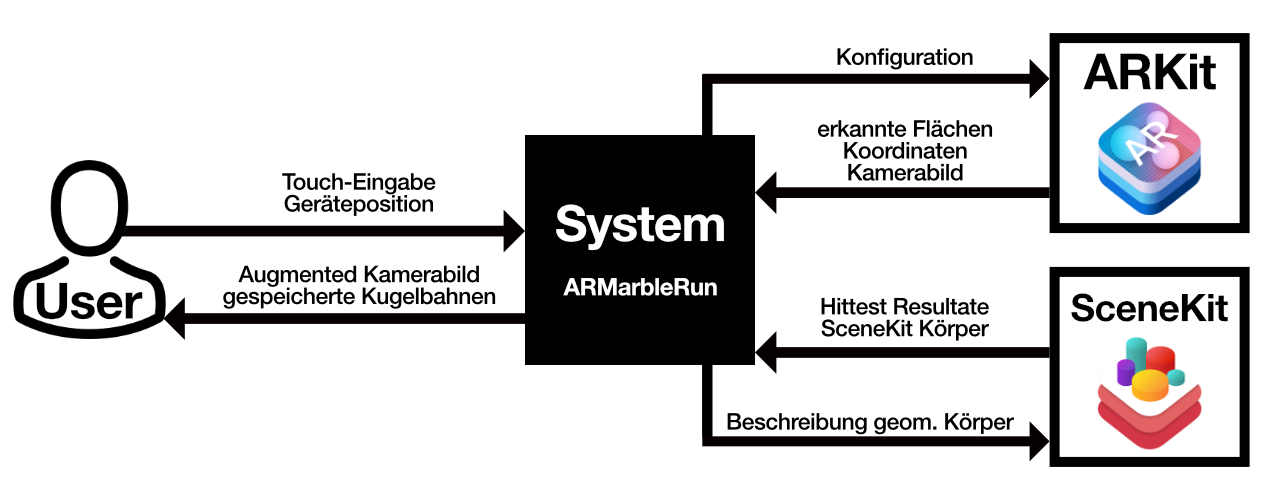
\includegraphics[width=\textwidth]{kontextdiagramm}
\end{figure}

\subsection{Systemvision}

Für Kugelbahnenthusiasten, cuboro Fans und solche die es noch werden wollen,
die ihre Kugelbahn mitnehmen wollen, planen wollen und nach Anleitung nachbauen wollen,
bietet unsere Kugelbahn App
mit Augmented Reality
eine komfortable, moderne und effiziente Methode seine Bahn zu planen oder zu bauen.
Anders als das offizielle cuboro Webkit,
ist die Kugelbahn mit der App mobil und man kann sie virtuell in einen realen Raum stellen.

\subsection{Architekturprinzipien}

Die zu entwickelnde Demo-App wird zu einem grossen Teil zum Selbstzweck erstellt.
Die App soll die ausgearbeiteten technologischen Möglichkeiten demonstrieren.
Der Code selber muss für an der entsprechenden Technik Interessierte hilfreich sein.
Dazu soll er informativ und verständlich sein.
Dies wird unter anderem mit \textbf{Selbstdokumentation} und der \textbf{Trennung von Verantwortlichkeiten} erreicht.
Die Trennung der Verantwortlichkeiten soll ausserdem dazu führen, dass einzelne Aufgaben/Teilprobleme gezielt studiert und wiederverwendet werden können.

\subsection{Taktiken}

Durch eine durchgehenden, starken Nutzung von Interfaces kann übersichtlich sichergestellt werden, welche Bestandteile der Software welche Aufgaben lösen. Die Interfaces sollen sprechene Methoden und Attributevariablen haben und wo notwendig mit Kommentaren ergänzt werden. Dieses Vorgehen hilft sowohl der Trennung von Verantwortlichkeiten und der Selbstdokumentation.

Weiter sollen Klassen möglichst klein und kohäsiv gehalten werden und zu zusammengehörigen Modulen gruppiert werden. Somit sollen interessante Stellen im Code rascher gefunden und verstanden werden. Das Vereinfacht die Wiederverwendung einzelner Module.

\subsection{Architekturstil}

Da die App monolithischen Charakter hat, also ohne Verbindungen nach Aussen und ohne Notwendigkeit zur Kommunikation mit verteilten Komponenten ist, fallen verteilte Stile (Client-Server, P2P usw.) weg.
Praktisch alle Abläufe in der App werden durch den Benutzer ausgelöst und führen zur Ausführung verschiedener Use Cases. Im Kern stehen die Kugelbahnen und deren Elemente.
Ein Stil nach dem Vorbild von Clean Architecture scheint daher passend zu sein: Events aus dem UI werden über Interfaces an verschiedene Interactor (Use Cases) weitergegeben, welche die Entities abrufen und bearbeiten.

Bei Recherchen stiessen wir auf die VIPER Architektur, welche versucht Clean Architecture spezifisch für iOS umzusetzen. Jeder Use Case ist ein VIPER Modul, das aus View, Interactor, Presenter, Entities und Wireframe (Router) besteht. Die Wireframes initialisieren ihr Modul und sind für das Aufrufen anderer Module verantwortlich. Der Interactor nutzt die globalen DataManager um Daten aufzurufen und für den Presenter bereitzustellen.

\begin{figure}
  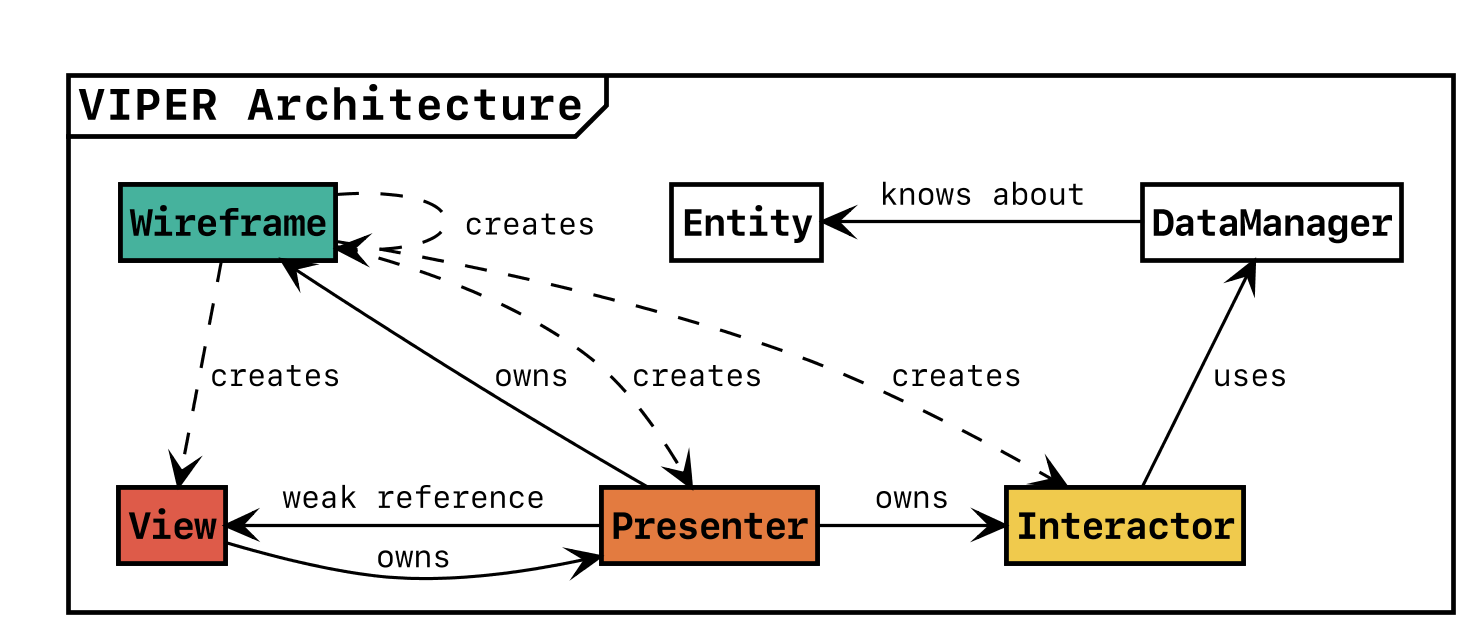
\includegraphics[width=0.8\textwidth]{viper-architecture}
\end{figure}

Die beiden wesentlichen Funktionen Bauanleitung (ARGuide) und Baumodus (AREditor) sind jeweils ein solches Modul. Sie teilen sich den DataManager, der Zugriff auf Kugelbahn- und Element-Entities hat. Daneben gibt es den Startbildschirm, bei dem der User den Modus wählen kann (SelectMode) und Listenansichten für Kugelbahnen (MarbleRunList) und Elemente (ElementList).

\begin{figure}
  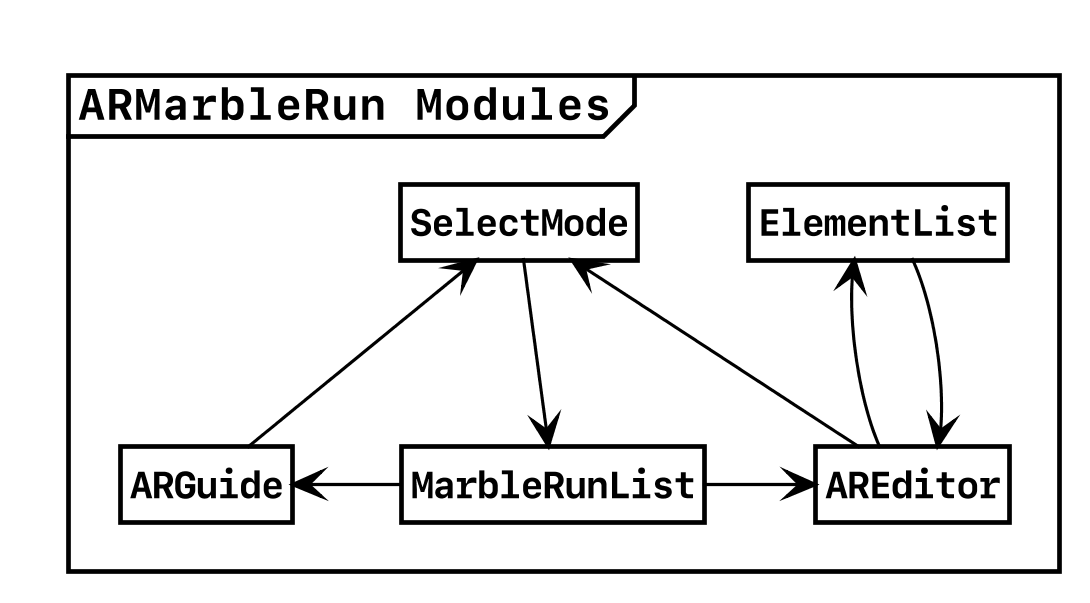
\includegraphics[width=0.5\textwidth]{viper-modules}
\end{figure}

\subsection{Systemsichten}

Alle Aktivitäten gehen von der View, bzw. vom Benutzer aus. Daher beginnt der folgende Fluss mit der View.

\begin{figure}
  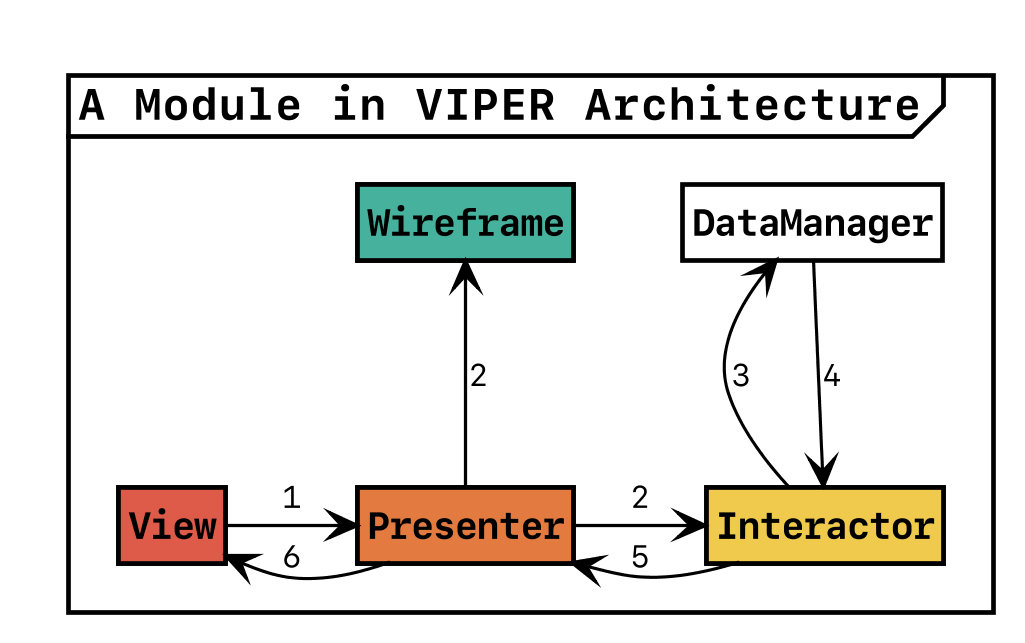
\includegraphics[width=0.5\textwidth]{viper-architecture-numbered}
\end{figure}

\begin{enumerate}
  \item Die View übergibt ein Event an den Presenter.
  \item Je nach Event wird entweder ein anderes Modul aufgerufen (via Wireframe) oder eine Anfrage nach Daten an den Interactor, der die Business Logik hat gerichtet.
  \item Der Interactor sendet einen Request nach Daten an den entsprechenden DataManager.
  \item Der DataManager gibt die gewünschten Entity Daten zurück.
  \item Der Interactor verarbeitet die Daten falls nötig und gibt sie an den Presenter weiter.
  \item Vom Presenter erhält die View nun Informationen, wie sie sich zu verändern hat.
\end{enumerate}

\subsection{Architekturentscheidungen}

Im folgenden zwei der wichtigsten Architekturentscheidungen:

\begin{table}
  \begin{tabular}{l p{13cm}}
    Issue         & 
      Der Benutzer soll zwischen den beiden Modi Baumodus und Bauanleitung wechseln können, ohne die virtuelle Kugelbahn neu im realen Raum zu platzieren. \\
    Alternatives  & 
      \begin{tabular}[t]{@{}p{13cm}@{}}
        Zwei Varianten:
        \begin{enumerate}
          \item Nur die relevanten UI Elemente (Buttons) ein-/ausblenden und eine Eventhandler Klasse verwenden, die ausgetauscht werden kann.
          \item Zwei getrenne Module machen, die sich die AR Szene mit den relevanten Informationen übergeben.
        \end{enumerate}
      \end{tabular} \vspace*{-\baselineskip}
      \\
    Outcome       & 2. Zwei getrennte Module. \\
    Rationale     &
      Eine saubere Trennung der unterschiedlichen Modi hilft der Nachvollziehbarkeit und Verständlichkeit des Codes und entkoppelt die Komponenten. Dies unterstützt ausserdem die Trennung der Verantwortlichkeiten und Erweiterbarkeit und bietet eine klarere Struktur. \\
  \end{tabular}
\end{table}

\begin{table}
  \begin{tabular}{l p{13cm}}
    Issue         &
      Die Elemente der aktuellen Kugelbahn müssen einerseits in der View als SceneKit Kindknoten der Kugelbahn zur Darstellung sein. Andererseits müssen sie in einem Konstrukt sein, das ihre logische Position und Nachbarn verwalten kann, um die Bauanleitung und Persistierung zu ermöglichen. \\
    Alternatives  &
      \begin{tabular}[t]{@{}p{13cm}@{}}
        Zwei Varianten:
        \begin{enumerate}
          \item Die SceneKit Knoten werden mit den notwendigen Informationen erweitert und zusammen mit logischen Koordinaten zusätzlich in einer Hashmap referenziert für die Business Logik.
          \item Die SceneKit Knoten werden rein auf ihre Funktion als UI Komponente reduziert und von zu persistierenden Entities getrennt.
        \end{enumerate}
      \end{tabular} \vspace*{-\baselineskip} \\
    Outcome       & 2. View und Entity trennen. \\
    Rationale     & 
      In Prototypen wurde Variante 1 versucht, dies führt jedoch zu starker Vermischung von Darstellung/View und der Business Logik. Die gewählte Variante stellt die Trennung von Verantwortlichkeiten sicher und erlaubt es zwischen der Darstellung von Persistierung von Kugelbahnen zu abstrahieren. Dadurch könnte das Datenformat geändert werden, ohne auch die Handhabung der 3D Element/Knoten komplett ändern zu müssen. \\
  \end{tabular}
\end{table}


}



